\documentclass{beamer}
\usefonttheme{professionalfonts}

\usepackage{forloop}
\usepackage{calc}
\usepackage{tikz}
\usepackage{pgfplots}
\usetikzlibrary{arrows,automata}

\author{alireza}
\title{How to code}
\institute{Islamic azad university}
\usetheme{AnnArbor}

\setbeamercolor{}{fg=brown}

\usepackage{listings}

\begin{document}
	\begin{frame}
		\maketitle
	\end{frame}
	

	\newcounter{x}
	\newcounter{y}
	\newcounter{z}

	\begin{frame}
		\begin{tabular}{||r||r|r|r|r|r|r|r|r|r|r||}\hline\hline

			\ &
			\forloop{x}{0}{\value{x} < 10}{
				\arabic{x} \ifthenelse{\value{x}<9}{&}{}
			}
			\\\hline\hline
			
			\forloop{y}{0}{\value{y} < 10}{
				
				\arabic{y} \ifthenelse{\value{y}<10}{&}{}
				
				\forloop{x}{0}{\value{x} < 10}{
					\setcounter{z}{\value{x}*\value{y}}
					\arabic{z} \ifthenelse{\value{x}<9}{&}{}
				}   
				
				\\\hline
			}
		\end{tabular}
	\end{frame}
	
	
	\defverbatim[colored]\mycode{%
		\begin{lstlisting}[frame=single, emph={cout}, emphstyle={\color{blue}}]
			cout << "Hello world!";
		\end{lstlisting}
	}

	\begin{frame}
		\mycode
	\end{frame}
	
	\begin{frame}
	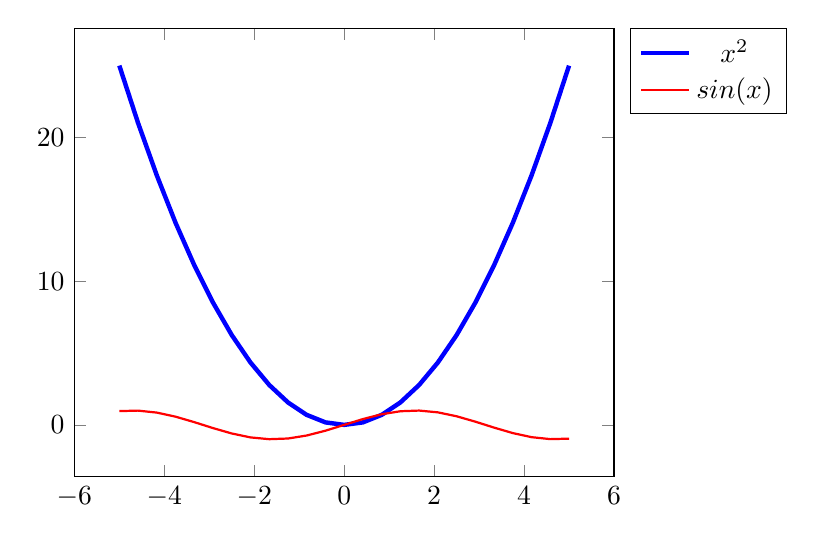
\begin{tikzpicture}
	\begin{axis}[domain=-5:5,legend pos=outer north east]
		\addplot[ultra thick,blue] {x^2};
		\addplot[thick,red] {sin(deg(x))};
		\legend{$x^2$, $sin(x)$}
	\end{axis}
	\end{tikzpicture}
	
	\end{frame}

	\begin{frame}
	
\begin{tikzpicture}
		\draw[fill=red] (1,0) -- (0,1) -- (-1,0) -- (0,-1) -- cycle;
	\end{tikzpicture}
	
	
\begin{tikzpicture}
		\draw (-3, -3) grid (3, 3);
	\end{tikzpicture}
	\end{frame}
	
	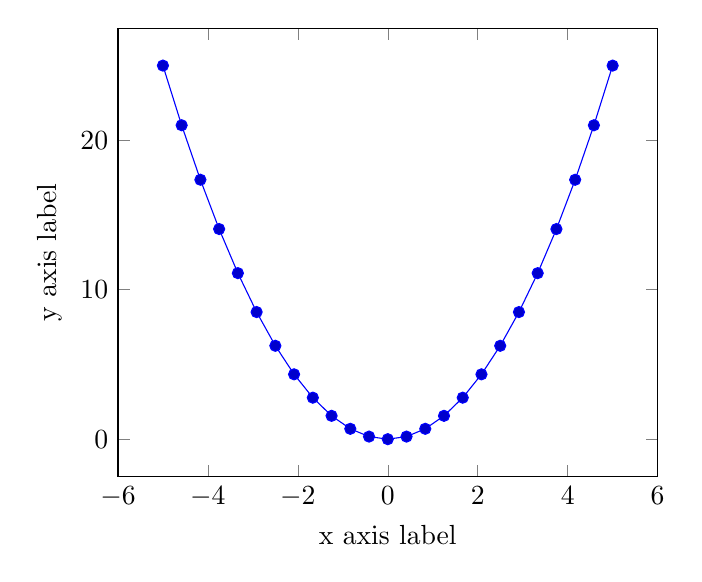
\begin{tikzpicture}
	\begin{axis}[xlabel=x axis label,ylabel=y axis label]
		\addplot {x^2};
	\end{axis}
	\end{tikzpicture}
\end{document}